\begin{figure}[b!]
\centering
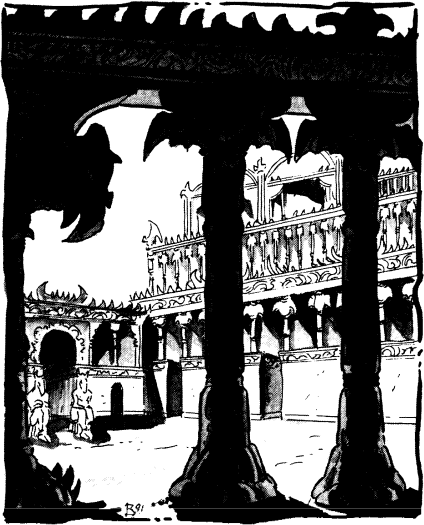
\includegraphics[width=\columnwidth]{images/nibenay-1.png}
\end{figure}

\City{Nibenay}
{24,000 (60\% humans, 12\% half-giants, 10\% dwarves, 10\% elves, 4\% half-elves, 3\% muls, 1\% other).}
{Rice, timber, hardwood, weapons, copper.}
{Common, Dwarven, Elven, Nibenese.}
{
	Nibenay has been affected by the monumental happenings of recent months, for the Shadow King has changed his approach to ruling the masses and dealing with the neighboring city-states. Like Hamanu and Lalali-Puy, Nibenay (who shares the same name as his domain) witnessed the deaths of the Dragon and the other sorcerer-kings.

	He saw Rajaat reach out from beyond the veil of Athas to wreak vengeance against those who betrayed him. He also saw Rajaat defeated by the efforts of lowly mortals from the city of Tyr. In the wake of these signs and portents, Nibenay realized it was time to reconsider how best to rule his city, for the time for change had come.

	The city-state of Nibenay is located east of Tyr at the northern tip of the Crescent Forest. It barely felt the effects of the Great Earthquake, as it was protected by the Windbreak Mountains. Nibenay has also thus far been spared from Tyr-storms and the growing unrest spreading throughout the Tablelands. If the Shadow King has his way, none of these problems will ever reach his domain.
}
{
	Though there have been no major changes to life in Nibenay, enough strange occurrences have been worked into the routine to put a different spin on the city-state. For example, average citizens and even powerful nobles never expected to see the Shadow King, let alone attend one of his courts. Now the Shadow King regularly makes public appearances and shows an active concern for his community. This doesn't mean that life is any harder or easier than it's always been. It's just different. If a citizen or visitor breaks a law and can't afford to bribe a templar, then that citizen or visitor is still going to end up in Nibenay's slave pens.

	The other major change is the city's outlook on matters of a martial nature. The Shadow King and his templars seem to be concentrating much of their efforts on bolstering Nibenay's military might. The army regularly practices in the arena and patrols of the surrounding countryside have increased dramatically. In addition, free citizens and nobles have been ordered to serve in Nibenay's defense. Templars are busy organizing them into part-time militias and regimenting training sessions.

	What the Shadow King is truly concerned about, besides the unrest and upheaval that seems to be spreading throughout the Tablelands, are the rumors claiming that Dregoth has returned. Nibenay knows how powerful the sorcerer-king of Giustenal was. Dregoth was second only to Borys the Dragon in power. If Dregoth and his city have somehow come back from the dead, Nibenay wants to be prepared.

	After all, Nibenay's city-state is one of the closest to the ruins of ancient Giustenal, and he has no intention of losing his domain to a rival that was destroyed two millennia ago.
}
{
\begin{figure*}[b!]
\centering
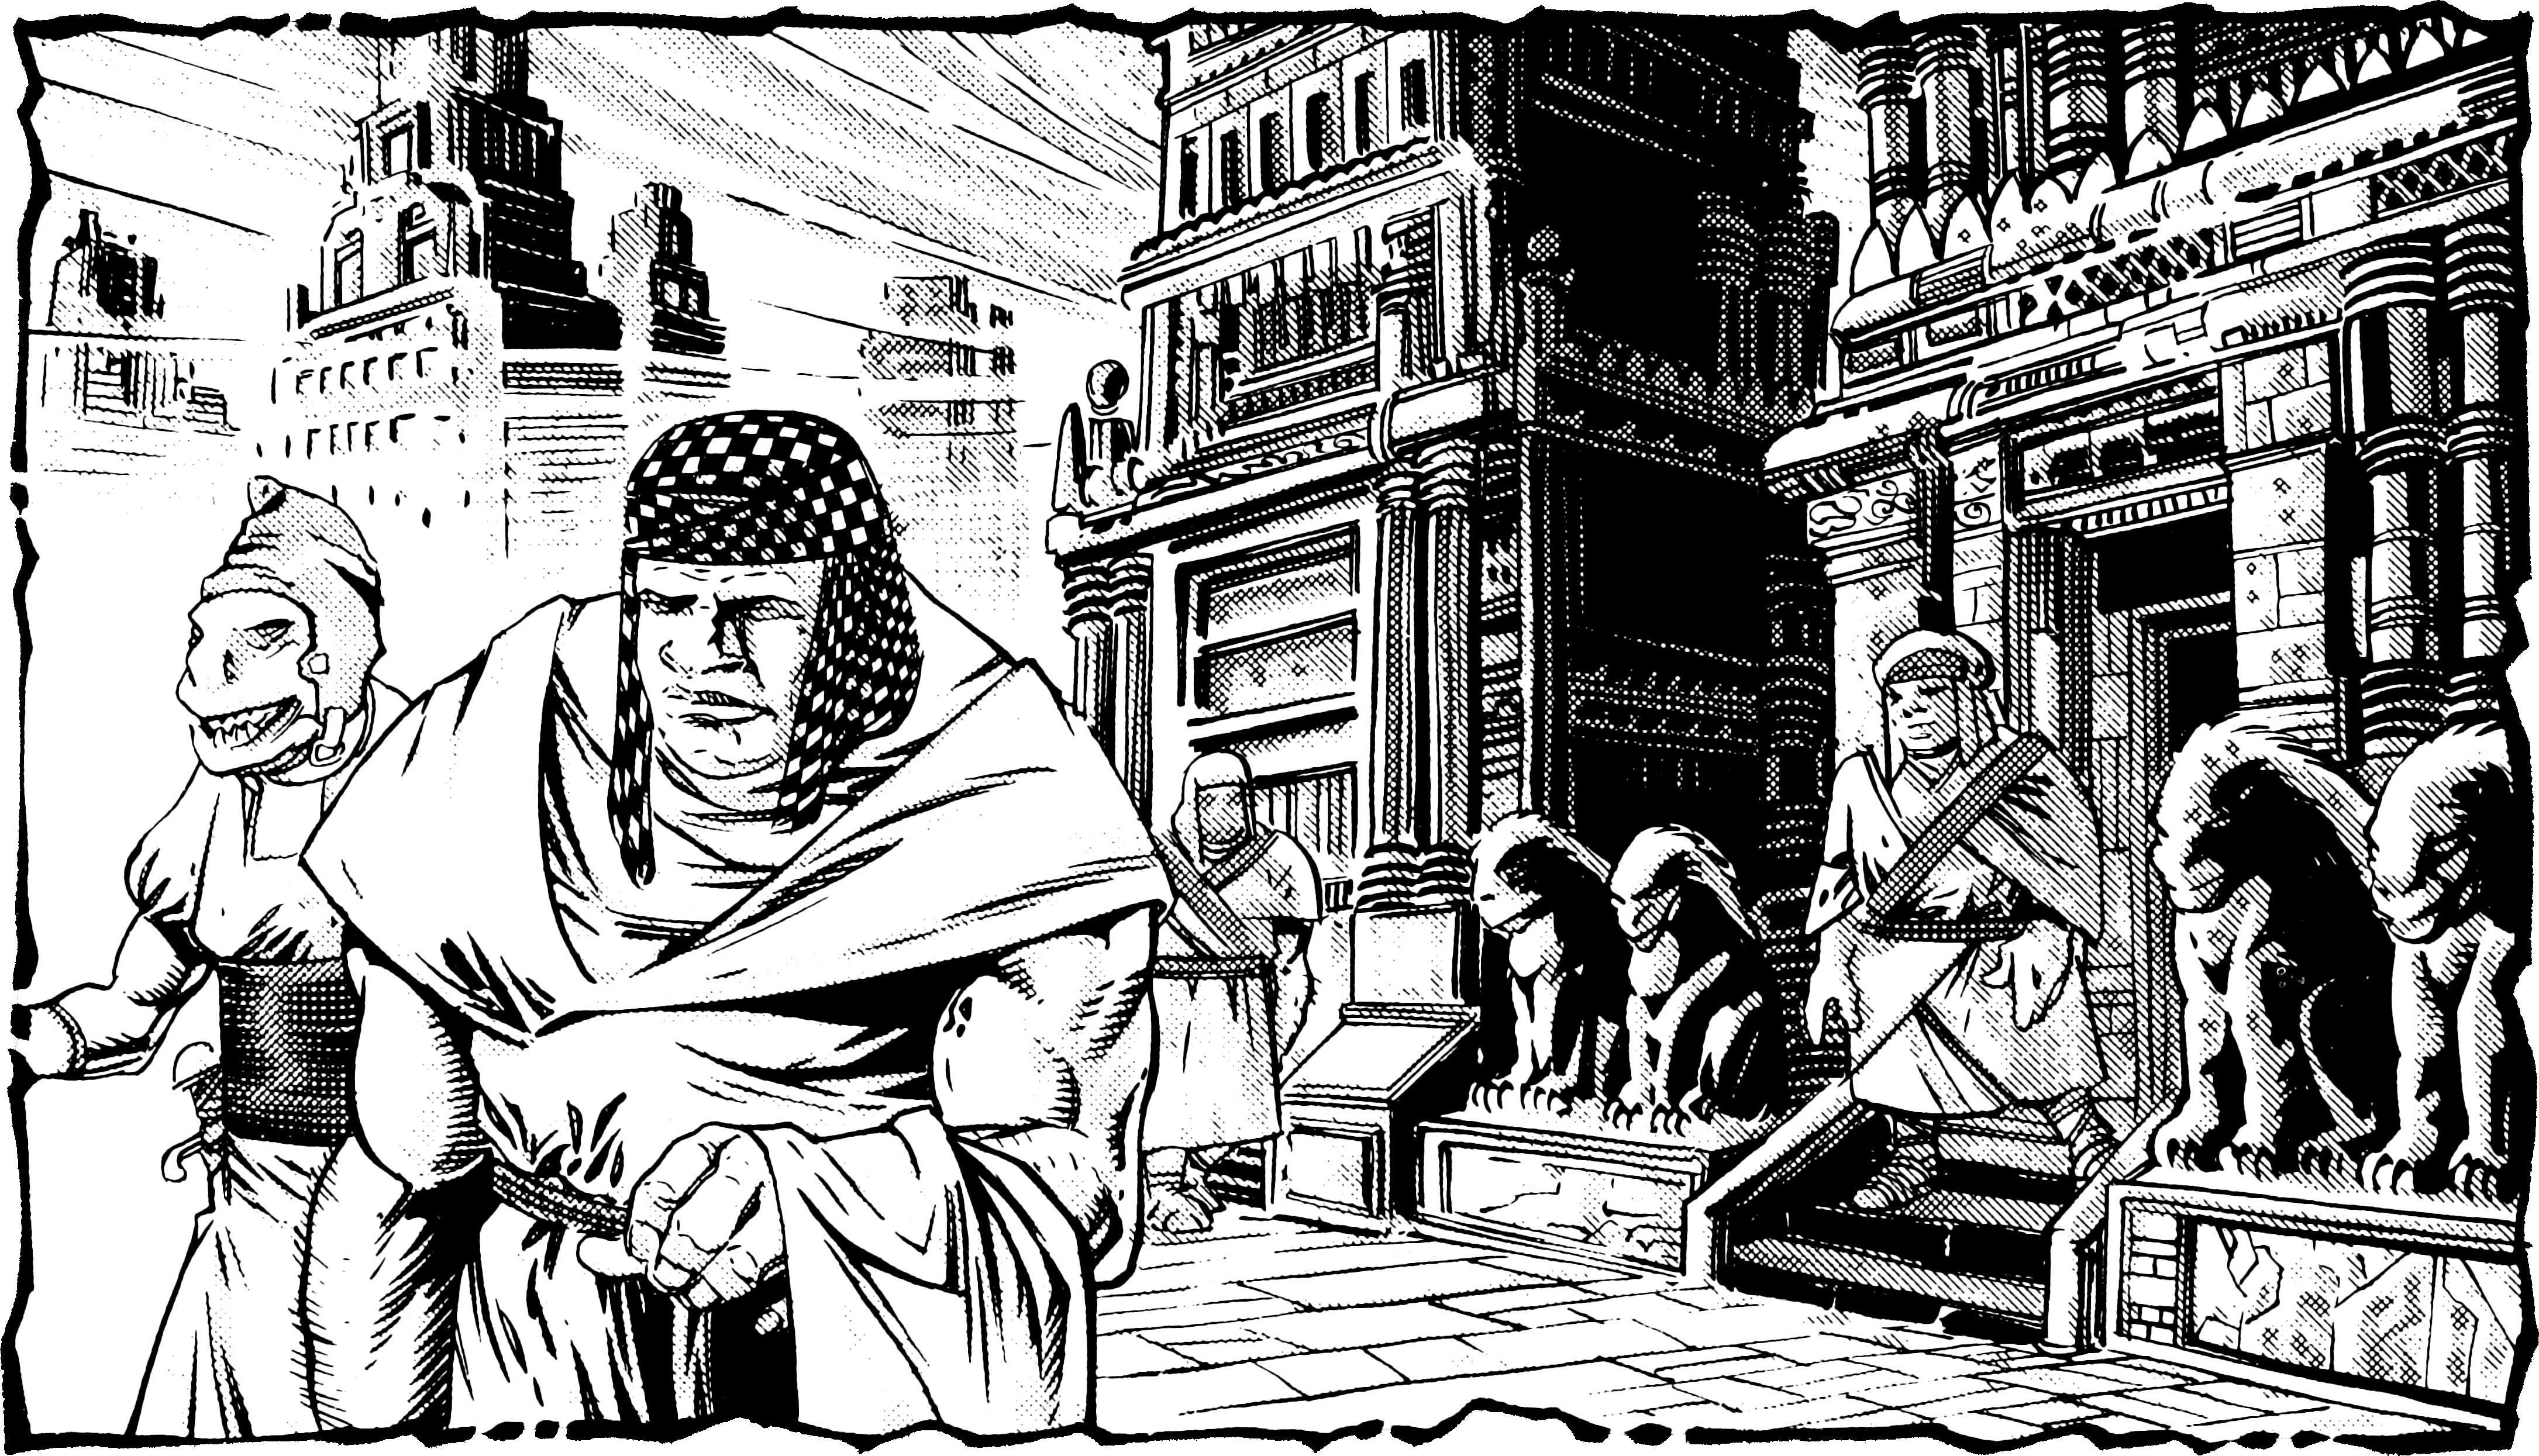
\includegraphics[width=\textwidth]{images/nibenay-2.png}
\end{figure*}

	The sorcerer-king Nibenay (LE male champion of Rajaat stage IV dragon, defiler 5/seer 5/loremaster 10/cerebremancer 10/Athasian dragon 2) used to stay behind the scenes. He was called the Shadow King because he rarely left Naggaramakam, his walled sub-city. His templars, who are all female, ran the city with skill and great care. Now, however, the Shadow King has become more prominent.

	In the past, the average free citizen could hope to see King Nibenay once or perhaps twice in an entire lifetime. Since the time of the Great Earthquake, Nibenay has taken a more active role. He still allows his templars to deal with the daily business of government, but now Nibenay has turned his attention away from the mysterious scholarly pursuits that once occupied his time to hold court for the city's nobles and free citizens.

	Nibenay's military might was never a question, but it also was never a major concern of the Shadow King. Now he actively seeks to understand his forces and looks for ways to improve their might and readiness. While the city used to appear to be secure in its own position, it now seems to be gearing up to battle an enemy that only the Shadow King knows about. The problem is that the enemy is change, and no army that Nibenay raises will be able to stop its relentless tide.

	In the wake of all this upheaval, Nibenay's nobles continue to care for and maintain the bubbling springs that surround the city. They don't know what to make of the Shadow King's sudden interest in the business of the city, but many of them are seeking ways to improve their own positions by getting closer to their once-elusive king.
}
{
	\textbf{Poortool's Horde}: Lead by the half-Elven preserver Poortool (LN male half-elf preserver 5/seer 3/cerebremancer 5), the Horde is a raiding tribe to the east of Nibenay. Poortool is a renegade from the Veiled Alliance who seeks to study magic without any restriction that the Veiled Alliance or sorcerer-king Nibenay may apply. He has created a community for likeminded preservers in a village in the foothills of the Black Spine Mountains. He has also allied with the gith of the Black Spine Mountains who provide guards and raiders for his tribe. Poortool seeks to make it difficult for members of the Veiled Alliance in Nibenay to convince its members to leave the Alliance and join him.

	\textbf{House Shom}: House Shom is thought to be the oldest merchant house operating in the Tyr region. For centuries the house amassed great wealth through aggressive trading. However, now the House is seen as passive and decadent. The Shom family members are almost never seen in public and have little to do with the daily business of the house. Instead the family members live decadent lives in their palaces, engaging in expensive parties and balls. The running of the trading house is left to the house agents. Most of the agents place their interests ahead of House Shom's interests, and there is much infighting between agents. This has lead to a decline in the House's prospects over the past few decades. Only the house's immense wealth has saved it from collapse already. House Shom is known to use non-human guards on its caravans and as raiders against other merchant houses, including thri-kreen packs and belgoi tribes. The house is currently ruled by Temmnya Shom (NE female human, defiler 15). Her younger brother, Jebea Shom (LN male human, rogue 3/fighter 2/dune trader 1) has begun a reform movement to straighten out the family's problems, but his popularity threatens Temmnya's position. She has contemplated disposing of him if she can do so without her involvement being discovered by other family members.

	\textbf{Sky Singers}: The Sky Singers elf tribe maintains a permanent market in the Hill District of Nibenay. It is the only known instance of a permanent Elven market. The market is filled with goods of all kinds from the rare to the common. The Sky Singers have a reputation of offering quality products that were not stolen from their previous owners, unlike most Elven tribes. While the tribe numbers over 3,000 members, much of the time the elves are off wandering, leaving only a dozen or so elves to tend the marketplace. But when the tribe returns, the Sky Singers' market takes on a festive atmosphere.

	\textbf{The Veiled Alliance}: Nibenay's Alliance has an utter hatred of defilers. This has led to a rare commodity beneath Athas' crimson sun-idealism. With the help of an ancient spiritual force known as the zwuun, which resides in the hot springs outside the city, the Alliance does what it can to protect wizards who use preserving magic. The Alliance doesn't feel it can oppose the Shadow King directly, so it directs its activities against lesser defilers. Thagya Phon (LN male human, preserver 7/veiled one 10) leads the Nibenese Alliance, though his health has begun to fail him in recent years. He has two goals he wishes to accomplish before he dies: He longs to discover what Nibenay's scholar slaves have been working on in the Naggaramakam, and he has a dream of mounting the Shadow King's head on the obsidian pedestal that rises from the floor of his spartan quarters.
}
{
	\textbf{Cromlin (Hamlet, 150)}: The trading village of Cromlin sits on the shores of the Silt Sea, northeast of Nibenay. House Shom runs the village, though House M'ke has a sizable operation as well. Together they handle the vast majority of trade from the north, as traders attempt to bypass the chaos of Raam. Cromlin traders use silt skimmers to navigate the silt shoals, keeping the trade route to Break Shore open. The shoal navigators of Cromlin are in high demand, for they are among the select few who can lead silt skimmers along the buried paths.

	Cromlin is a wild place, full of people who are too untamable to live in the cities. Thieves of all sorts reside in the village. Silt pirates use it as a haven and other scoundrels and restless souls are drawn to its sandy shores. Master trader Hurdll Crost (N male human, bard 10/dune trader 5) and his agents turn a blind eye towards shady characters as long as they remain to do business in his village.

	\textbf{Salt View (Small Village, 550)}: Nestled in the Mekillot Mountains, Salt View is a chaotic sprawl of tents and buildings located within a large cavern on the mountain's eastern face. Ex-slaves of all races fill the community. The tribe originally practiced raiding as its primary occupation, but today it is known for a lavish form of storytelling called theater. Salt View's traveling theater troupes are welcome across the Tyr Region, though they present themselves as free merchants from the independent House Fyra (a cover for Salt View activities). The troupes perform for caravans, at oasis villages, and even in the city-states of Tyr, Nibenay, and Balic.

	\textbf{Vavrek (Thorp, 200)}: Vavrek is typical of the small farming villages located throughout the Fertile Crescent. The village is located southwest of Nibenay within sight of the Crescent Forest. The villagers grow vegetables, mostly soybeans. The land the village is built on is owned by the Koelse noble family, to which the villagers must pay rent. The village is administered by a templar-wife of Nibenay named Sonyalah (NE female human, templar 5/wife of Nibenay 3).
}
{
	\textbf{The City Reservoir}: The Shadow King had this enormous stone cistern constructed centuries ago to supply the city with water in the event of a siege. The top of the reservoir is covered and a lush garden, maintained by the templars, grows on top of the reservoir.

	\textbf{The Coliseum}: The coliseum rises above the dilapidated buildings in a rundown part of the city. The size of the arena is immense, taking up four city blocks and rising six stories high. It is an ancient building and it is said that not even the Shadow King knows when the coliseum was built and by whom. Elaborate carvings and etchings cover the coliseum's stonework. The square shaped arena floor stretches almost a quarter of a mile across.

	\textbf{Monasteries of the Exalted Path and of the Serene Bliss}: Nibenay has a tradition of monasteries. The two orders are called the Exalted Path and the Serene Bliss. The monks pledge loyalty to the King and their teachings include the quiet acceptance of authority, so the templars tolerate them. They are treated with great respect by the citizens. The monks live very aesthetic lives, tending gardens and mediating. Many of the monks, especially those of the Exalted Path, study psionics. The Exalted Path consists entirely of male monks and is led by Thong Nal, (CN male human, air cleric 3) who encourages the study of psionics at his monastery. Other monks become artisans who specialize in the carving of the images that cover the buildings of Nibenay. The Serene Bliss is an all female order and is led by the abbess Au Treng (LN female human, cleric 4).

	\textbf{Naggaramakam}: The Naggaramakam is a walled forbidden inner city where the sorcerer-king Nibenay lives with his templar-wives. Only templars are permitted to enter and leave the Naggaramakam. While slaves are permitted to be brought into the Naggaramakam, once inside they are never allowed to leave. No free citizen is ever allowed to see the inside of the Naggaramakam. The sorcerer-king's palace is said to be carved into a stone relief of the Shadow King with dancing women, representing his templar-wives, strung together as if they were his hair.

	\textbf{The Omnipotent Receivers}: A line of large statues of sorcerer-king Nibenay stand on each side of the main road leading to the city. The statues are called the Omnipotent Receivers as it is believed that King Nibenay sees all that the statues see.

	\textbf{The Plain of Burning Water}: The city of Nibenay is situated on the border of a large area of hot springs. Called the Plain of Burning Water, the hot springs provide the water needed by the citizens of Nibenay. Each noble house owns at least one of the hot springs which is the source of much of the wealth of the nobility.

	\textbf{Sage's Square}: Sage's Square is the largest open area inside of the city. The grand emporiums of all the dynastic merchant houses are located around the square and are the center of trade in Nibenay, where almost anything can be purchased. The square was named Sage's Square because scholars and sages use to gather under the shadow of the huge agafari trees that grew in the square, and debate philosophy. This tradition ended only a few years ago when a renegade defiler, fleeing the templars defiled the trees. King Nibenay had the dead trees removed from the square, and ordered that no other trees be planted in the square as a public reminder of the danger of renegade defilers.

	\textbf{The School of Augurs}: The school of Augurs is the largest school for psionic instruction in Nibenay. The head master is a dwarf named Djef, who developed a scheme to help support the school by hiring out its students to transfer telepathic messages and to teleport-deliver small parcels.
}
{
	\item A disguised dray agent has entered Nibenay seeking to make contact with nobles disgruntled with the Shadow-King's rule. The dray tries to gather together as many nobles as possible so that when Dregoth makes his attack on Raam, he can start a rebellion in Nibenay to distract the Shadow-King from interfering in Dregoth's plan.
	\item The templars attempt to ambush a cell leader of the Veiled Alliance who they believe is staying at the same inn as the PCs. During the templar raid, one of the PCs is mistakenly identified as the Veiled Alliance member. Capture means execution, so the PCs must flee. If the PC makes it out of the city, his problems are not over. Because of the secrecy of the Veiled Alliance, the subordinates of the cell leader have never met him before. When the templars identify the PC as the cell leader, the other members assume it to be true. When the PC flees the city the cell members attempt to enforce Requital, believing the PC has tried to resign from the Veiled Alliance.
	\item Ramai is a templar of Nibenay, who is responsible for interrogations. Dedicated and highly skilled in all manner of interrogation and torture techniques, she holds some respect within the templar hierarchy. Her career appeared promising until one day, inexplicably, Ramai fell in love with one of her victims, a young man named Tongkol. Unable to bear the thought of Tongkol suffering under torture but also realistic enough to know they can never be together, she assigns the PCs the task of spiriting Tongkol out of the city. Ramai will not offer the PCs any direct help, but can give them information to help them succeed. If the PCs fail and are captured, Ramai will deny any involvement with the PCs and see that they are executed quickly to silence them.
	\item Gith raiders have discovered a previously unknown ancient catacomb that allows them to enter the city undetected. They raid some dwellings in the city and attempt to flee back the way they came. But undead that were angered by the gith's trespass have arisen and prevented the gith from getting out of the catacombs. The PCs are sent into the catacombs after the gith and must also face the undead horrors.
	\item One of House Shom's merchant forts has been overrun by gith. The PCs are hired to lead the assault to retake the desert fortress.
	\item A preserver of the Veiled Alliance asked the zwuun for help on his latest research. The zwunn's answer directed the preserver to the site of ancient ruins that overlook the road to North Ledopolus where he could find what he sought. Unsure if the zwuun was being mischievous or not, the preserver sends the PCs to scout out the ruins.
}